
\chapter{Overview of Optimization Methods \label{chap:02-Optimization_models}}

% First paragraph has no indentation.

\noindent Optimization may be informally defined as the procedure
of finding better solutions to a given problem that usually models
some physical phenomenon. In our every day life, we are constantly
solving small optimization problems, like choosing the shortest route
to a friend's house, or organizing the appointments in our agenda.
In general, these problems are small enough for us to find a good
solution without extra help, but as they become larger and more complex,
the aid of computers for their resolution is unavoidable.

Complex multidimensional optimization problems are popular in engineering,
economics, physics and other scientific fields. When solving an optimization
problem, the objective is to find a ``good'' solution in a ``reasonable''
computational time. In this respect, the field of mathematical optimization
has received a lot of attention by the scientific community during
the last decades. However, both ``good'' and ``reasonable'' are
problem, application and context-specific concepts, in which the biggest
challenge of selecting an appropriate optimization approach usually
lays.

Mathematical optimization involves the process of finding solutions
from a group of possible decisions, which may be defined as:

\begin{equation}
\min f(\vec{x})\qquad\vec{x}\in\Omega\subseteq\mathbb{R}^{n},
\end{equation}


\noindent where $\vec{x}=(x_{1},\dots,x_{n})$ is a vector representing
the decision variables, $f(\vec{x})$ is the objective function measuring
the quality of the decisions and $\Omega$ is the set of possible
solutions of the problem, also known as search space. Note that the
objective function $f$ makes it possible to define a total order
relation between any pair of solutions in $\Omega$.

The search space $\Omega$ may also be expressed as a solution to
a system of equations or inequalities, e.g.:

\begin{eqnarray}
g(x_{1},\dots,x_{n}) & \leq & 0\nonumber \\
h(x_{1},\dots,x_{n}) & = & 0.
\end{eqnarray}


Optimization problems involving the maximization of the objective
function also fall into this category, since:

\begin{equation}
\max f(\vec{x})=-\min(-f(\vec{x})).\label{eq:02-maximization_minization_problem_relation}
\end{equation}


A point $\vec{x}^{*}$ is considered to be an unrestricted local minimum
of a function $f$ if it holds a better value than all its neighbors,
i.e., there exits $\epsilon>0$ so that:

\begin{equation}
f(\vec{x}^{*})\le f(\vec{x})\qquad\forall\vec{x}\in\mathbb{R}^{n}\qquad\mid\vec{x}-\vec{x}^{*}\mid<\epsilon.\label{eq:02-local_minimum}
\end{equation}


\noindent Similarly, a point $\vec{x}^{*}$ is considered to be an
unrestricted global minimum of a function $f$ if it holds a better
value than all others, i.e.:

\begin{equation}
f(\vec{x}^{*})\leq f(\vec{x})\qquad\forall\vec{x}\in\mathbb{R}^{n}.\label{eq:02-global_minimum}
\end{equation}


The concepts of local and global minimum are considered strict if
the inequalities of Equations~\ref{eq:02-local_minimum} and~\ref{eq:02-global_minimum}
are strict. Likewise, the definition of local and global maximum is
given by the existing relation between a minimization and a maximization
problem, as specified in Equation~\ref{eq:02-maximization_minization_problem_relation},
i.e., a point $\vec{x}^{*}$ is a local or global maximum of a function
$f$ if and only if $\vec{x}^{*}$ is a local or global minimum of
function $-f$, respectively.


\section{Gradient-based methods \label{sec:02-Gradient-based-methods}}

Gradient-based methods are among the oldest and most studied optimization
approaches. They are based on the derivative of the optimized function,
using the first and even the second derivative of a function $f$.
The name gradient follows from the derivative of multidimensional
functions, $\nabla f(\vec{x})$, which is simply a vector where each
element is the slope of $\vec{x}$ in that dimension, i.e., $<\frac{\partial f}{\partial x_{1}},\dots,\frac{\partial f}{\partial x_{n}}>$~\cite{Luke-Essentials_of_metaheuristics:2009}.

The principle behind gradient-based methods is rather simple. Starting
from an arbitrary value for $x$, a subtraction (or addition) of a
small positive value is iteratively applied to it, e.g., for gradient
descent:

\begin{equation}
x\leftarrow x-\alpha f'(x),
\end{equation}


\noindent where $\alpha$ is a small positive value, and $f'(x)$
is the first derivative of $f(x)$. Consequently, a positive slope
will make $x$ decrease, whereas a negative slope will make it increase.
Figure~\ref{fig:02-gradient_descent} shows an example of this behavior.
Therefore, $x$ will gradually move down the function until it finds
its minimum, where $f'(x)$ is zero, causing it to stop.

\begin{figure}
\centering

\includegraphics[width=0.55\textwidth]{02-background_and_motivation/img/gradient_descent}

\caption{Gradient descent with a negative slope, i.e. $x$ is increasing. \label{fig:02-gradient_descent}}
\end{figure}


However, gradient methods have certain drawbacks that make them unsuitable
for tackling a wide range of optimization problems. Take, for example,
the time they take to converge. As gradient descent approaches a function
minimum, it will skip this point and land on the other side. In the
next step, something similar will happen, but this time from the other
side of the minimum point, thus slowly approaching to the target in
a ``zig-zag'' way. This behavior is directly related to the slope
of the function at the given point, i.e., a steepest slope translates
into a larger jump, and may be alleviated by adjusting the value of
$\alpha$. However, some functions (or regions of functions) may require
smaller values, while for others, a bigger value would be more appropriate.
Newton's method improves this by taking the second derivative of the
function, $f''(x)$, into account, i.e.:

\begin{equation}
x\leftarrow x-\alpha\frac{f'(x)}{f''(x)},
\end{equation}


\noindent thus adjusting the value of $\alpha$ as it converges towards
a point with zero slope \cite{Luke-Essentials_of_metaheuristics:2009}.

Another issue is how other points are handled. Beside maxima and minima
points, some functions also contain saddle points (known as inflection
points in one-dimensional functions). Clearly, the first derivative
of a saddle point is zero, meaning gradient descent will stop looking
for the minimum, even though it has not found it (see Figure~\ref{fig:02-gradient_descent_saddle_point}).
Newton's method, on the other hand, does not help either, even trying
to divide by zero in this case. These observations clearly show how
gradient methods get caught in local optima. Local optima of a function
are defined as the optima (or minima in this case) of a local region.
Similarly, global optima are defined as the optima of the whole domain
of a function. It follows that gradient methods, as gradient descent
or Newton\textquoteright{}s method, are local optimization algorithms
\cite{Luke-Essentials_of_metaheuristics:2009}.

\begin{figure}
\centering

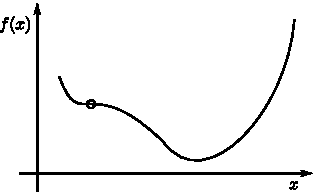
\includegraphics[width=0.55\textwidth]{02-background_and_motivation/img/gradient_descent_saddle_point}

\caption{A saddle point or point of inflection, where the derivative is zero.
\label{fig:02-gradient_descent_saddle_point}}
\end{figure}


But maybe the biggest concern with gradient-based methods is that
they assume the function under optimization is derivable. This assumption
holds only when optimizing a well-formed mathematical function. Unfortunately,
this is generally not true, since in most cases, the gradient is not
computable because the function is not known. The only available approach
in such situations is creating inputs to the function in order to
assess their quality. Metaheuristics (see Section~\ref{sec:02-Metaheuristics})
are good candidates for this class of problems, for solving both moderate
and large instances.


\section{Linear and non-linear programming}

It was in the early 40s of the twentieth century, through the work
of teams formed by mathematicians, economists and physicists, that
the bases were established for the resolution of problems with a set
of techniques known as linear and non-linear programming. Their initial
goal was to solve different kinds of logistic problems during the
second world war.

In a linear programming optimization problem, both the objective function
$f$ and a given set of constraints are linear functions. The constraints
impose restrictions over $\vec{x}$, i.e., they must meet certain
requirements as, for example, fulfill a limited availability of resources.
A problem may be formulated as follows:

\begin{equation}
\min f(\vec{x})=c\cdot\vec{x}\label{eq:02-linear_programming_objective_function}
\end{equation}


\noindent subject to

\begin{eqnarray}
A\cdot\vec{x} & \le & b\nonumber \\
\vec{x} & \ge & \vec{0}.\label{eq:02-linear_programming_constraints}
\end{eqnarray}


\noindent In the example above, the inequalities defined in \ref{eq:02-linear_programming_constraints}
are the constraints to the linear program defined in \ref{eq:02-linear_programming_objective_function}.

For solving continuous, linear-optimization problems, efficient exact
algorithms exist, such as the simplex method \cite{Dantzig-Maximization_of_a_linear_function_of_variables_subject_to_linear_inequalities:1951}
or the interior-points method \cite{Karmarkar-A_new_polynomial_time_algorithm_for_linear_programming:1984}.
Indeed, linear programming is one of the most satisfactory models
for solving optimization problems, since the feasible region of the
problem is a convex set and the objective function is a convex function.
It follows that the global optimum is a node of the polytope representing
the feasible region \cite{Talbi_Metaheuristics:2009}. See Figure
\ref{fig:02-linear_programming_example} for a linear-programming
example with several constraints.

\begin{figure}
\centering

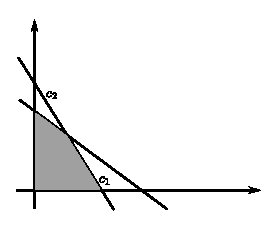
\includegraphics[width=0.55\textwidth]{02-background_and_motivation/img/linear_programming}

\caption{Graphical representation of a linear-programming example with two
constraints, $c_{1}$ and $c_{2}$. The grayed area is the polytope
representing the region of feasible solutions. \label{fig:02-linear_programming_example}}
\end{figure}


Non-linear programming models, on the other hand, consider problems
where the objective function $f$ and/or the constraints are non-linear
\cite{Bazaraa-Nonlinear_programming:2006}. However, non-linear continuous
problems are more difficult to solve. Despite several existing techniques
to linearize such models, they often not only introduce extra variables
and constraints, but also some degree of approximation \cite{Glover-Improved_linear_programming_formulations_for_nonlinear_problems:1975}.
Moreover, some problem properties such as high dimensionality, parameter
interaction, and multi-modality make these approaches ineffective.

\bigskip{}


Generally speaking, when dealing with real-world problems, the availability
of analytical optimization models, such as those required by gradient
methods or (non-)linear programming, is not guaranteed. Indeed, for
some applications, only simulations or physical models are the available
means for objective-function evaluation \cite{Fu-Optimization_for_simulation:2002}.
Once again, metaheuristics appear as good candidates to solve different
instance sizes of this class of problems. 


\section{Metaheuristics \label{sec:02-Metaheuristics}}

Metaheuristics, a term proposed by Glover in \cite{Glover-Future_paths_for_integer_programming_and_links_to_artificial_intelligence:1986},
represent a group of approximation algorithms designed to combine
basic, heuristic principles with advanced high-level guidance methods,
targeted at improving the efficiency of a search process. These techniques
are meant to find good solutions to a given problem, for which the
mathematical function is not available or its search space is big
enough for an exhaustive search to be unfeasible~\cite{Kochenberger_Handbook_of_metaheuristics:2003}.

From the theoretical point of view, metaheuristics represent a subset
of stochastic optimization, since they use some degree of randomness
to find optimal (or as good as possible) solutions to hard problems.
They are the most general of this kind of algorithms, and are applied
to a wide range of problems~\cite{Luke-Essentials_of_metaheuristics:2009}.
Unlike the exact optimization methods introduced in the previous sections,
metaheuristics do not generally guarantee the optimality of the obtained
solutions~\cite{Talbi_Metaheuristics:2009}. Moreover, they do not
define how close the obtained solutions are from the optimal ones,
as approximation algorithms do.

The characterization given by Blum and Roli~\cite{Blum-Metaheuristics_in_combinatorial_optimization_overview_and_coconceptual_comparison:2003}
provides a clear overview of the fundamental properties associated
with metaheuristics:
\begin{itemize}
\item metaheuristics are strategies that \textquotedblleft{}guide\textquotedblright{}
the search process;
\item their goal is to efficiently explore the search space in order to
find optimal or near-optimal solutions;
\item they build upon techniques which range from simple local search procedures
to complex learning processes;
\item they are approximate and usually non-deterministic;
\item they may incorporate mechanisms to avoid getting trapped in confined
areas of the search space;
\item their basic concepts permit an abstract-level description, which is
not problem-specific;
\item they may make use of domain-specific knowledge in the form of heuristics
that are controlled by the upper level strategy;
\item advanced metaheuristics use search experience (implemented as some
form of memory) to guide the search process.
\end{itemize}
The strategies used by metaheuristics should provide a dynamic balance
between the exploitation of the accumulated search experience (commonly
called intensification) and the exploration of the search space (commonly
called diversification)~\cite{Blum-Metaheuristics_in_combinatorial_optimization_overview_and_coconceptual_comparison:2003}.
This balance provides the necessary means to quickly identify promising
regions, and early discarding those which have already been explored
or do not provide solutions of better quality. Promising regions within
the search space, which are identified by the obtained ``good''
solutions, are thoughtfully explored during the intensification phase,
hoping to find better solutions. On the other hand, during the diversification
phase, not-yet-visited regions are explored, making sure the search
space as a whole is evenly explored, thus confining the search to
a reduced number of regions is avoided. In this context, the ultimate
search algorithm in terms of diversification is random search. Random
search generates a random solution in the search space at each iteration,
without using memory~\cite{Talbi_Metaheuristics:2009}. In terms
of intensification, iterated local search~\cite{Lourencco-Iterated_local_search:2003}
is a representative algorithm. The steepest local search algorithm
selects, at each iteration, the best neighboring solution that improves
the current one~\cite{Talbi_Metaheuristics:2009}.

Metaheuristics are applicable where state-of-the-art exact algorithms
cannot tackle the given instances within the required time, either
because of their size or structure. The meaning of ``required time''
within this context directly depends on the target optimization problem
itself. A feasible or acceptable time may vary from some seconds to
several months, again, depending on the target optimization problem,
e.g., real-time decisions against structural-design problems.

Based on the characterization given by Talbi~\cite{Talbi_Metaheuristics:2009},
a summary of the essential properties of optimization problems that
justify the use of metaheuristics follows:
\begin{itemize}
\item Very large problem instances. Even though exact polynomial-time algorithms
might be known for solving the target problem, they are too expensive
due to the size of the instances.
\item Problems with hard real-time constraints, where a ``good solution''
has to be found online. Metaheuristics appear as an alternative to
exact algorithms in order to reduce the search time.
\item A difficult problem of moderate size, which input instances have an
intricate structure.
\item Optimization problems with time-consuming objective function(s) and/or
constraints. Indeed, various real-world optimization problems are
characterized by the huge computational cost of the objective functions.
Several radio-network design problems fall into this category.
\item Problems that cannot be solved with exhaustive search due to the non-analytical
models on which they are based. These problems are defined by a black-box
evaluation of the objective function (see Section~\ref{sub:02-Black_box_optimization}).
\end{itemize}
The influence of these conditions may increase in the presence of
non-deterministic optimization models, e.g., problems with complex
Monte Carlo simulations~\cite{Creutz-Microcanonincal_monte_carlo_simulation:1983}.

Undoubtedly, metaheuristics are rapidly gaining popularity as optimization
problems are increasing in both size and complexity. Indeed, as the
computing power of commodity hardware increases, the possibility of
building models of greater complexity is available for developing
more accurate models of real-world problems in engineering and science.

\bigskip{}


Related literature groups metaheuristic algorithms due to their behavior,
for example:
\begin{itemize}
\item differential evolution, from the family of evolutionary algorithms;
\item differential ant-stigmergy algorithm, from the family of swarm-intelligence
algorithms; and
\item simulated annealing, from the group of classic metaheuristic algorithms. 
\end{itemize}
Each of these algorithms minimize an objective-function value by adopting
essentially distinct approaches. In the following sections, a short
description of their functioning is given.


\subsection{Differential evolution \label{sub:02-DE}}

Differential Evolution~(DE\nomenclature[A]{DE}{Differential evolution})~\cite{storn1997_Differential_evolution}
is a simple and powerful evolutionary algorithm proposed for numerical
optimization. The version of DE used for this thesis is known as DE/rand/1/bin,
or \textquotedbl{}classic DE\textquotedbl{}~\cite{Price-Differential_evolution_a_practical_approach:2005}.
At the beginning, the classic DE initializes a population of $N$,
$D$-dimensional vectors with parameter values that are distributed
with random uniformity between pre-specified lower and upper initial
parameter bounds, $x_{i,\mathrm{{low}}}$ and $x_{i,\mathrm{{high}}}$,
respectively~\cite{Ronkkonen-Real_parameter_optimization_with_differential_evolution:2005},
i.e.:

\begin{eqnarray}
x_{i,j,g} & = & x_{i,\mathrm{{low}}}+\mathrm{{uniform}[0,1)}\cdot(x_{i,\mathrm{{high}}}-x_{i,\mathrm{{low}}}),\nonumber \\
i & = & (1,2,...,D),\, j=(1,2,...,N),\, g=0.\label{eq:02-DE_structure}
\end{eqnarray}


\noindent In Equation~(\ref{eq:02-DE_structure}), $g$\nomenclature[S]{$g$}{Generation index in DE}
denotes the generation index, while $i$ and $j$ indicate the parameter
and population indices, respectively. Consequently, $x_{i,j,g}$ is
the $i^{\mathrm{th}}$ parameter of the $j^{\mathrm{th}}$ population
vector in generation $g$. The (pseudo)-random number generator is
represented by a function ``$\mathrm{{uniform}[0,1)}$''\nomenclature[S]{$\mathrm{{uniform}[0,1)}$}{Function representing a uniformly-distributed random number from the interval [0,1)}
that selects a uniformly-distributed random number from the interval
$[0,1)$.

DE generates solutions by applying the mutation and cross-over operations.
A vector from the current population is mutated by adding the scaled
difference of two other vectors from the same population, combined
with the mutation-scale factor. A proportion of the parameters of
the mutated vector are crossed with those belonging to the $j^{\mathrm{th}}$
population vector, resulting in a new solution vector. The cross-over
constant controls the proportion of parameters that the mutant vector
contributes to the new vector.

The generated solution vector is retained if it yields a lower objective-function
value than the $j^{\mathrm{th}}$ population vector, otherwise the
$j^{\mathrm{th}}$ vector is kept for at least one more generation.

The four parameters to control the search process of DE are: the population
size ($NP$\nomenclature[S]{$NP$}{Population size in DE}), the number
of generations for the algorithm to run ($g_{\mathrm{max}}$\nomenclature[S]{$g_{\mathrm{max}}$}{Number of generations for DE to run}),
the crossover constant ($CR$\nomenclature[S]{$CR$}{Crossover constant in DE}),
and the mutation scaling factor ($F$\nomenclature[S]{$F$}{Mutation scaling factor in DE}).

An extensive description of DE and its variants may be found in~\cite{Price-Differential_evolution_a_practical_approach:2005}.
A wide range of optimization problems have been solved by applying
DE~\cite{das2010_differential_evolution_state_of_the_art}, also
in the area of radio-network optimization~\cite{Benedicic_Balancing_downlink_uplink_soft_handover_areas_in_UMTS_networks:2012,DaSilva-Analysis_of_parameter_settings_for_differential_evolution:2008,Mendes-A_differencial_evolution_algorithm_to_optimize_the_radio_network_design:2006}.


\subsection{Differential ant-stigmergy algorithm \label{sub:02-DASA}}

The Differential Ant-Stigmergy Algorithm~(DASA\nomenclature[A]{DASA}{Differential ant-stigmergy algorithm})~\cite{korosec2010_DASA}
is based on the metaheuristic Ant-Colony Optimization (ACO\nomenclature[A]{ACO}{Ant-colony optimization})~\cite{dorigo2006ant_colony_optimization}.
ACO was pioneered by Dorigo in 1992 and is based on the foraging behavior
of social ants, which use pheromone as a chemical messenger. When
looking for a food source, a swarm of ants interacts in their local
environment. An ant is able to follow the route marked with pheromone
laid by other ants. When an ant finds a food source, it will mark
the trail to and from it with pheromone.

The pheromone concentration, $p$, evaporates at a constant rate,
$\rho$ , over time, $t$, i.e.:

\begin{equation}
p(t)=p_{0}\mathrm{e}^{-\rho t},\label{eq:02-ACO_structure}
\end{equation}


\noindent where $p_{0}$ is the initial pheromone concentration at
$t=0$. The evaporation is important, as it provides the means for
algorithm convergence and self-organization.

The pheromone concentration varies over time and the ants follow the
route with higher concentration. In turn, the pheromone concentration
increases with the number of ants. That is, as more and more ants
follow the same route, it becomes the favored path, producing a positive
feedback mechanism. Consequently, as the system evolves in time, it
converges to a self-organized state, which is the essence of any ant-based
algorithm. 

\bigskip{}


As it was mentioned before, DASA is an ant-based algorithm that provides
a framework to successfully cope with high-dimensional numerical optimization
problems. It creates a fine-grained discrete form of the search space,
representing it as a graph. This graph is then used as the walking
paths for the ants, which iteratively improve the temporary best solution. 

At the end of every iteration, and after all the ants have created
solutions, they are evaluated to establish if any of them is better
than the best solution found so far.

There are six parameters that control the way DASA explores the search
space: the number of ants ($m$\nomenclature[S]{$m$}{Number of ants in DASA}),
the discrete base ($b$\nomenclature[S]{$b$}{Discrete base in DASA}),
the pheromone dispersion factor ($\rho$\nomenclature[S]{$\rho$}{Pheromone dispersion factor in DASA}),
the global scale-increasing factor ($s_{+}$\nomenclature[S]{$s_{+}$}{Global scale-increasing factor in DASA}),
the global scale-decreasing factor ($s_{-}$\nomenclature[S]{$s_{-}$}{Global scale-decreasing factor in DASA}),
and the maximum parameter precision ($\epsilon$\nomenclature[S]{$\epsilon$}{Maximum parameter precision in DASA}).

A more in-depth explanation about these parameters and the DASA algorithm
itself can be found in~\cite{korosec2010_DASA}.


\subsection{Simulated annealing \label{sub:02-SA}}

This metaheuristic was introduced in the area of combinatorial optimization
by Kirkpatrick et al.~\cite{Kirkpatrick_OptimizationBySimulatesAnnealing}.
The algorithm resembles the physical annealing process, where particles
of a solid material arrange themselves into a thermal equilibrium.
Simulated Annealing~(SA\nomenclature[A]{SA}{Simulated annealing})
is based on the principle of local-search heuristics, and uses a pre-defined
neighborhood structure on the search space $\Omega$. The temperature
parameter controls the search behavior. Its name follows the analogy
to the physical annealing process. In each iteration, a solution $y$,
which is a neighbor of the current solution $x$, is computed. If
$y$ has a better objective-function value than $x$, it becomes the
new solution, i.e., the current solution $x$ is replaced by $y$.
If, on the other hand, $y$ has a worse objective-function value than
$x$, it is only accepted with a certain probability depending on
two factors: 
\begin{itemize}
\item the difference of the objective-function values of $x$ and $y$,
and
\item the temperature parameter. 
\end{itemize}
Intensification in SA is provided by the local-search nature of the
algorithm, while diversification is produced with non-zero temperatures,
by \textquoteleft{}\textquoteleft{}uphill\textquoteright{}\textquoteright{}
moves. The pseudo-code of the SA metaheuristic can be represented
as in Algorithm~\ref{alg:07-SA_pseudocode}. In this pseudo-code,
$T_{1},T_{2},...$ represent an usually decreasing sequence of values
for the temperature parameter, and ``$\mathrm{{uniform}[0,1]}$''
is a function for selecting a uniformly-distributed random number
from the given interval, whereas the meaning of the rest of the symbols
is as defined above.

\begin{algorithm}
\centering

\caption{Pseudo-code of the simulated-annealing metaheuristic. Adapted from~\cite{Bianchi-A_survey_on_metaheuristics_for_stachastic_combinatorial_optimization:2009}.\textit{\label{alg:07-SA_pseudocode}}}


\begin{algorithmic}
\Require $x \gets$ initial solution
\Require $T_{\mathrm{1}} \gets$ temperature parameter
\For {k=1,2,...}
	\State $y \gets$ random solution from $\Omega$
	\If {$f(y) \le f(x)$}
		\State $x \gets y$
	\ElsIf {$e^{(\frac{f(x)-f(y)}{T_{k}})} \le \mathrm{uniform}[0,1]$}
		\State $x \gets y$
	\EndIf
	\State $T_{k+1} \gets$ update temperature $T_{k}$
\EndFor
\end{algorithmic}
\end{algorithm}


SA has two parameters to control the search process: the initial temperature
($t_{\mathrm{initial}}$\nomenclature[S]{$t_{\mathrm{initial}}$}{Initial temperature in SA})
and the total number of iterations or evaluations ($it$\nomenclature[S]{$it$}{Maximum number of iterations in SA}).
SA also allows to define the way the temperature is lowered during
the annealing process.

SA has proved to be a solid optimization algorithm, capable of giving
high-quality solutions to a wide scope of optimization problems~\cite{Suman_SurveyOfSimulatedAnnealing}.
Additionally, several works employ the SA metaheuristic for solving
optimization problems in the area of radio network~\cite{Benedicic_Balancing_downlink_uplink_soft_handover_areas_in_UMTS_networks:2012,Duque-Channel_assignment_for_cellular_radio_using_simulated_annealing:1993,GarciaLozano_CPICHPowerOptimisationByMeansOfSimulatedAnnealingInAnUTRAFDDEnvironment,minimum.set.covering.problem:2000,Coverage.optimization.on.CPICH.tilt.and.azimuth:2006,Zhang-Mathematical_modelling_and_comparisons_of_heuristics_for_WCDMA_radio_planning:2006}.
A detailed description of SA and its applications can be found in~\cite{Van-Simulated_annealing:1987}.


\section{Black-box optimization \label{sub:02-Black_box_optimization}}

The complexity of a problem is equivalent to the complexity of the
best known algorithm solving that problem~\cite{Talbi_Metaheuristics:2009}.
If there exists a polynomial-time algorithm to solve a problem, the
problem is said to be easy or tractable. Similarly, if a problem is
difficult or intractable, there is no known polynomial-time algorithm
to solve it. 

Many optimization problems cannot be formulated with a clear analytical
mathematical notation. In such cases, the objective function may become
a black box \cite{Kargupta-Search_blackbox_optimization_and_sample_complexity:1996}.
This is one of the main advantages when using metaheuristics, i.e.,
there is no need of a complete knowledge of the targeted model. Indeed,
in a black-box optimization, no analytical formulation of the objective
exists~\cite{Talbi_Metaheuristics:2009}, as Figure \ref{fig:02-black_box_optimization}
shows.

\begin{figure}
\centering

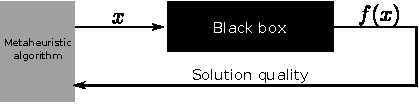
\includegraphics[width=0.55\textwidth]{02-background_and_motivation/img/blackbox_optimization}

\caption{A metaheuristic algorithm process using a black box for the objective-function
evaluation, $f(x)$, of a solution, $x$. \label{fig:02-black_box_optimization}}
\end{figure}


More specifically, a function $f(\vec{x})$, $\vec{x}\in\mathbb{R}^{n}$,
is a black-box function if and only if~\cite{Talbi_Metaheuristics:2009}:
\begin{itemize}
\item the domain $\vec{x}$ is known,
\item it is possible to get the value of $f$ for each $\vec{x}$ based
on simulation, and
\item there is no other information available for function $f$.
\end{itemize}
Typically, the experiments associated with this kind of problems are
very expensive in terms of time and cost, since a simulation must
be forced to evaluate the solution. Generally speaking, the most time-consuming
part of a metaheuristic optimization process is the evaluation of
the objective function~\cite{Talbi_Metaheuristics:2009}. This is
especially true when dealing with real-world problems of areas such
as structural design~\cite{Barthelemy-Approximation_concepts_for_optimum_structural_design:1993},
molecular docking~\cite{Tantar-A_parallel_hybrid_genetic_algorithm_for_protein_structure_prediction:2007}
and, the field on which this thesis focuses, radio-network design~\cite{Benedicic_Pilot.power.optimization:2010,Benedicic_Balancing_downlink_uplink_soft_handover_areas_in_UMTS_networks:2012,Benedicic-A_GPU_based_parallel_agent_optimization_approach:2013,Benedicic-A_GRASS_GIS_parallel_module_for_radio-propagation_predictions:2013,Benedicic-An_adaptable_parallel_simulation_framework_for_LTE_coverage_planning:2013}.
A possible substitution for lengthy evaluations is to reduce their
complexity by approximating the objective function, thus replacing
it with an approximation during the optimization process. This approach
is known as meta-modeling~\cite{Talbi_Metaheuristics:2009}. However,
when dealing with approximations, some degree of solution quality
is inevitably sacrificed. As it will be shown in the following chapters,
there is a very fine balance between the number of evaluations and
the quality of the achieved solutions. Consequently, reducing the
time spent in objective-function evaluation should favorably influence
the solution quality achieved by a preferred metaheuristic algorithm.
A major portion of this thesis is dedicated to improve this specific
aspect in the area of radio-network optimization, starting with a
high-performance, unified framework for radio-network planning, which
is presented in Chapter~\ref{chap:04-Framework-design-and-implementation}.

\bigskip{}


In practice, however, the black-box evaluation of the objective function
presents a problem. In the context of research about radio-network
optimization there is an inherent difficulty of providing the black-box
used to evaluate a given approach. A quick review of the state-of-the-art
in radio-network optimization indicates that this fact has become
increasingly popular in several published works~\cite{Amaldi-Radio_planning_and_coverage_optimization_of_3G_networks:2008,chen2008automated,Chen-Fast_algorithm_for_large_scale_UMTS_coverage_planning:2009,Antenna.azimuth.tilt:2009,Antenna.Configuration:2008,Siomina:Minimum.pilot.power.for.service.coverage}.
Clearly, this fact creates a barrier to one of the most important
phases of scientific methodology: experimental reproducibility~\cite{gauch2002scientific}. 

There are several reasons behind this situation. For example, it is
a known fact that proprietary software, providing good computational
models for radio-network simulation, is a very expensive tool for
science. Even neglecting the economical aspect, but considering the
great variety of software packages and license combinations, it is
practically impossible for a research laboratory to have the whole
palette of commercially-available solutions at its disposal. Moreover,
genuine users of these applications are generally not allowed to mention
the formats, protocols, or algorithms used by the proprietary software,
since their disclosure is often explicitly forbidden by restrictive
licenses.

Some non-commercial and open-source packages for radio-network simulation~\cite{Ozimek_Open.source.radio.coverage.prediction:2010,Momentum.project,Mehlfuhrer_The_Vienna_LTE_Simulators_enabling_reproducibility_in_wireless_communications_research:2011,Pillekeit-A_hybrid_simulation_framework_for_the_evaluation_of_common_RRM:2012,Piro_Simulating_LTE_cellular_systems_an_open_source_framework:2011,Yeung-Detailed_OFDM_modeling_in_network_simulation:2004}
present two main drawbacks: poor documentation and/or low scalability.
The scalability issues shown by some projects prevent these packages
to be used in larger, real-world environments, where big problem instances
are the rule. Despite this, the merit and acknowledgment go to the
authors of these frameworks, not only for providing them to the scientific
community, but fundamentally because of providing an environment in
which different kinds of simulations are completely reproducible.
Additionally, the lack of documentation represents a big hurdle for
extending the base code, which becomes a difficult task without the
help of the original authors of the package. In such cases, author's
knowledge is required for effectively expanding the functionality
of an open-source tool. This is especially true when dealing with
complex simulation frameworks, as the ones used for radio networks.


\chapter{Principles of Mobile Radio Networks \label{chap:02-Principles_of_mobile_radio_networks}}

A cellular mobile radio network is a collection of individual cells
that are served by several transmitters, called Base Stations~(BSs\nomenclature[A]{BS}{Base station}).
Each BS gives radio coverage to a small geographical area. The integration
of the coverage of various BSs provides radio coverage over a much
larger geographical area, thus defining a cellular radio network.
The two basic functions of a radio-network system are: 
\begin{itemize}
\item to locate and track both active and idle mobile devices, called User
Equipments~(UEs\nomenclature[A]{UE}{User equipment}); and
\item to attempt to connect each UE to the best available BS.
\end{itemize}
The first task involves a location-update procedure, which allows
a UE to inform the network about its movement from one location area
to the next. This process is called mobility management. The second
task requires the constant evaluation of the radio-link quality with
the serving BS, and the radio-link qualities of alternate BSs. This
process is called radio-resource management, and is performed by the
network using knowledge about the link-quality evaluations of the
reference channels, e.g., the pilot channels.

The radio communications between a UE and a grid of BSs use low power.
However, the movement of the UE causes highly irregular radio-link
conditions, thus consistent monitoring and precise control are required
to keep the radio-link quality at an acceptable level. At the core
of the evaluation of radio-link quality is a statistical-measurement
process based on a previous knowledge of the expected characteristics
of the pilot channel. On the one hand, the link quality, and the size
and distribution of the cells of a modern radio cellular system are
limited by the speed of the link-quality measurement and network control.
On the other hand, the spectral efficiency of a radio network is bounded
by the cell sizes, the ability of radio links to withstand interference,
and the ability of the system to react to variations in traffic~\cite{Stuber-Principles_of_mobile_communication:2011}.

Cellular radio systems partition the available spectrum among the
BSs, and a given frequency is reused at the closest possible distance
that the radio link will allow. Consequently, smaller cells have a
shorter distance between reused frequencies, and this results in an
increased spectral efficiency and traffic-carrying capacity. The radio
links of a high-capacity radio network interfere with each other due
to frequency reuse. For this reason, it is always desirable to use
the lowest possible transmit power while maintaining each radio link
above a given Quality-of-Service~(QoS\nomenclature[A]{QoS}{Quality of service})
threshold. Therefore, radio links should not significantly exceed
their target QoS, since doing so will cause unnecessary interference
to other radio links~\cite{Stuber-Principles_of_mobile_communication:2011}.
This particular situation is further discussed in Chapter~\ref{chap:06-Experimental-evaluation-the-service-coverage-problem},
where an optimization approach that minimizes the total transmit power
used in a radio network is presented.


\section{Handover \label{sub:02-Handover-and-soft-handover}}

In radio networks, handover (or handoff) is one of the main features
that allows the mobility of UEs~\cite{WCDMAforUMTS_RadioAccessForThirdGenerationMobileCommunications}.
The concept behind the handover operation is simple: when a UE moves
from the coverage area of a cell to the coverage area of a neighboring
cell, the system creates a new connection with the latter cell and
disconnects the user from the former one, so that an acceptable link
quality can be maintained. Otherwise, the increase in transmit power
that is required to compensate for path loss results in excessive
interference. The handover procedure consists of two processes~\cite{Stuber-Principles_of_mobile_communication:2011}:
\begin{itemize}
\item the link-quality evaluation before handover initiation, and
\item the allocation of radio and network resources.
\end{itemize}
Generally speaking, radio networks with smaller cell sizes require
faster and more reliable handover algorithms. Indeed, it has been
shown that the number of cell-boundary crossings is inversely proportional
to the cell size~\cite{Labedz-Handover_control_issues:1987}. Since
there is certain probability of dropping a connection whenever a handover
is attempted, it is clear that the role of handover configuration
becomes more important as the cell sizes decrease. Therefore, if the
radio network does not detect poor signal quality fast enough, or
makes too many handovers, the capacity is diminished due to increased
interference and/or excessive control traffic~\cite{Stuber-Principles_of_mobile_communication:2011}.


\subsection{Hard handover}

During a hard handover, a UE can connect to only one BS at a time.
A unique decision initiates and executes a handover without making
a number of simultaneous connections among candidate BSs. Based on
link measurements, the target BS is selected prior to executing the
handover, and the active connection is instantly transferred to it.
Moreover, the connection even experiences a brief interruption during
the actual transfer, because the UE can only connect to one BS at
a time. In contrast to soft handover (see next section), hard handovers
do not take advantage of the diversity gain, where the signals from
two or more BSs arrive at comparable strengths. Hard handover is a
simple and inexpensive way to support UE mobility. It is used in Time-Division,
Multiple-Access (TDMA\nomenclature[A]{TDMA}{Time division multiple access})
cellular systems such as GSM~\cite{Stuber-Principles_of_mobile_communication:2011}.


\subsection{Soft handover}

Soft Handover~(SHO\nomenclature[A]{SHO}{Soft handover}) enhances
handover functionality by allowing a UE to potentially operate on
multiple radio links at a time (see Figure~\ref{fig:02-SHO_example}).
During SHO, the target BS is selected as the best candidate from among
the available BSs. The UE performs the necessary link-quality measurements
by monitoring the signals from the surrounding BSs. Simultaneously
keeping multiple connections means that SHO enhances the system performance
through diversity reception.

Despite the advantages it provides, SHO is complex and expensive to
implement. Additionally, interference actually increases with SHO,
since several BSs can connect to the same UE. This increase in forward
interference can become a problem. If the handover region is large,
such that there are many UEs in SHO mode, the increased interference
due to several BSs connected to the same UE can become a problem~\cite{Stuber-Principles_of_mobile_communication:2011}.

The SHO procedure is important in systems using the channel-access
method known as Code Division Multiple Access~(CDMA\nomenclature[A]{CDMA}{Code division multiple access}),
and especially in the Wideband CDMA~(WCDMA\nomenclature[A]{WCDMA}{Wideband code division multiple access}),
which is employed by the UMTS. CDMA systems are interference-limited
meaning their capacities are closely related to the level of interference
they can tolerate. Specifically, a CDMA system cell is affected by
the interference within its own cell, and also interference from its
neighboring cells. In order to mitigate the level of interference,
and thus increase the capacity and quality, CDMA systems use power
control. The main idea behind power control is to prevent the UEs
and the BSs from transmitting more power than is strictly necessary
to meet the target QoS level. For the power control to work properly,
the system must ensure that each UE is connected to the BS having
the least attenuation at all times. If this is not the case, a positive-feedback
problem appears, and it can potentially destabilize the entire system~\cite{Wong-Soft_handoffs_in_CDMA_mobile_systems:1997}.
The SHO procedure helps to prevent such situations by ensuring that
each UE is served by the best BS most of the time, i.e., by allowing
connections to multiple BSs.

\begin{figure}
\centering

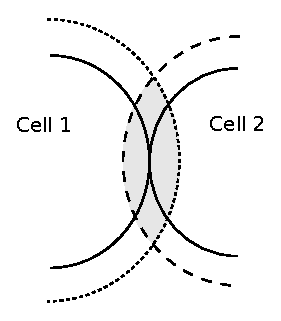
\includegraphics[width=0.3\textwidth]{02-background_and_motivation/img/sho_example}

\caption{An example of the soft-handover region, showed as a grayed area. The
area boundaries are configurable relative to the pilot-signal level
of each cell. Adapted from~\cite{Stuber-Principles_of_mobile_communication:2011}.
\label{fig:02-SHO_example}}
\end{figure}


The SHO condition depends on the relative, received-signal quality
from different cells and the SHO window, which triggers the addition
of a cell to the active set of the UE. Depending on radio propagation
characteristics, the radio transmission can gain more than 3~dB out
of a SHO situation~\cite{WCDMAforUMTS_RadioAccessForThirdGenerationMobileCommunications}.
From this point of view, SHO is a method to reduce interference and
improve radio quality, particularly at the cell border where the radio
coverage is of inferior quality. In UMTS Release 99~\cite{WCDMAforUMTS_RadioAccessForThirdGenerationMobileCommunications},
SHO is specified to work from the BS towards the UE (downlink), and
from the UE towards the BS (uplink).

With the introduction of the High Speed Packet Access~(HSPA\nomenclature[A]{HSPA}{High speed packet access})
as an improvement of the performance existing in WCDMA protocols,
the role SHO plays in mobile network configuration and functioning
slightly changed. The key difference is that the High Speed Downlink
Packet Access~(HSDPA\nomenclature[A]{HSDPA}{High speed downlink packet access})
does not support SHO, whereas the High Speed Uplink Packet Access~(HSUPA\nomenclature[A]{HSUPA}{High speed uplink packet access})
does. This particular distinction is further discussed in Chapter~\ref{chap:07-Experimental-evaluation-the-SHO-alignment-problem},
because it has some important implications in the balanced distribution
of SHO areas, and thus in the quality and capacity of HSPA services~\cite{holma2006hsdpa}.


\chapter{Overview of Radio-Network Optimization \label{chap:02-Optimization_of_radio_networks}}

Once a radio network is launched, an important part of its operation
and maintenance deals with monitoring its quality characteristics.
With the evolution of mobile communications, the complexity of network
planning has grown along with its throughput capacity, thus making
it practically impossible to plan modern radio networks with traditional
methods. In this sense, an examination of colored coverage maps in
conjunction with some statistical analysis are no longer appropriate
tools for troubleshooting a network. Moreover, since real-world radio
networks are large and many of their configuration parameters are
interdependent, an engineer is not able to cope with the level of
complexity present in these systems. For this reason, the computer,
along with specialized software, guides the engineer to the most appropriate
configuration for the network. In the context of this thesis, this
process is referred to as radio-network optimization.

Radio-network optimization may be divided into two fundamental phases:
analysis and decision~\cite{Nawrocki-Understanding_UMTS_radio_network_modelling_and_optimisation:2006}.
The analysis phase consists of the examination of the network performance,
which mainly focuses on the definition and collection of Key-Performance
Indicators (KPIs\nomenclature[A]{KPI}{Key performance indicator}).
KPIs are quantifiable measurements that reflect different network-quality
factors. The second phase deals with the decision making, based on
the analytical results collected in the previous phase, about changing
a particular configuration or parameter setting. The process, a representation
of which is depicted in Figure~\ref{fig:Optimization-cycle}, is
repeated until the achieved results are acceptable. Notice the similarity
with the general, decision-making process that was presented in Chapter~\ref{chap:01-Introduction},
Figure~\ref{fig:01-decision_making_process}.

\begin{figure}[h]
\centering

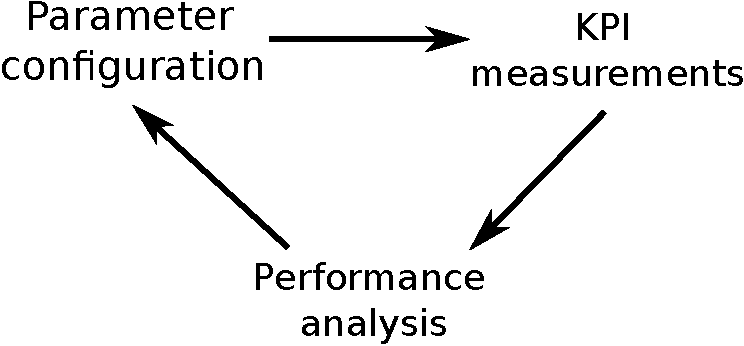
\includegraphics[width=0.4\textwidth]{02-background_and_motivation/img/optimization_cycle}

\caption{A typical optimization cycle for radio networks. This sequence is
repeated until the achieved results are acceptable. \label{fig:Optimization-cycle}}
\end{figure}


\bigskip{}


Since radio networks are increasingly more sophisticated, the need
for optimization methods that are capable of dealing with greater
complexity is far from declining. Indeed, several radio-network optimization
problems were shown to be NP-hard, since the computational time grows
non-polynomially with the problem size~\cite{Amaldi-Planning_UMTS_base_station_locations:2003,Amaldi-Radio_planning_and_coverage_optimization_of_3G_networks:2008,Gordejuela-LTE_access_network_planning_and_optimization:2009,Han-Optimizing_cell_size_for_energy_saving_in_cellular_networks:2012,Lee-Proportional_fair_frequency_domain_packet_scheduling_for_LTE_uplink:2009,Razavi-Performance_improvement_of_LTE_tracking_area_design:2008,Siomina:Minimum.pilot.power.for.service.coverage}.
As described in~\cite{Nawrocki-Understanding_UMTS_radio_network_modelling_and_optimisation:2006},
there are other reasons directly related with the growth of already
deployed networks that also increase the need for optimization methods:
\begin{description}
\item [{Network~performance~improvement}] more users receive service
coverage with the same physical infrastructure, making parameter optimization
the less expensive and only viable short-term approach.
\item [{Changes~in~user~profile}] the introduction of new, faster services
puts additional stress on the infrastructure, requiring additional
optimization efforts.
\item [{Changes~in~the~propagation~conditions}] the allocation of different
frequency bands for different systems, e.g., GSM, UMTS or LTE, requires
the deployment of new BSs, the radio propagations of which behave
differently, especially in urban areas.
\end{description}
Depending on the optimization problem being addressed, network operators
define an optimization target that is represented by an objective
function that maps possible configurations into a real value. Unfortunately,
there is no universal objective function in the field of radio-network
optimization~\cite{Nawrocki-Understanding_UMTS_radio_network_modelling_and_optimisation:2006}.
However, it is possible to optimize for a different target at a time,
such as service coverage, SHO balance or signal propagation. Particular
optimization algorithms for solving these problems are presented in
Chapters~\ref{chap:06-Experimental-evaluation-the-service-coverage-problem},
\ref{chap:07-Experimental-evaluation-the-SHO-alignment-problem} and~\ref{chap:05-Framework_parameter_tuning},
respectively. In all three cases, the introduced optimization approaches
are performed ``offline'', meaning that the optimization software
is not an active part of the target radio network. As the feedback
information of each optimization target, the statistical data about
the network functioning is used.

\bigskip{}


Bellow, an overview of some well-known optimization problems for radio-mobile
networks is given. Each section describes an optimization problem,
and presents a short survey of recently proposed optimization methods
for solving them.


\section{Optimizing base-station locations}

Some authors~\cite{minimum.set.covering.problem:1997,minimum.set.covering.problem:2000}
formulate the problem of locating BSs in terms of the minimum set-covering
problem (see Figure~\ref{fig:02-Minimum_set_covering_problem}).
The set-covering problem is defined by considering the signal level
in every test point from all BSs and requiring that at least one level
is above a fixed threshold.

\begin{figure}[H]
\centering

\begin{minipage}[c]{0.45\textwidth}%
\centering

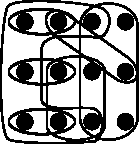
\includegraphics[width=0.6\textwidth]{02-background_and_motivation/img/set_covering-IN}

(a)%
\end{minipage}\hfill{}%
\begin{minipage}[c]{0.45\textwidth}%
\centering

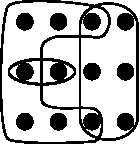
\includegraphics[width=0.6\textwidth]{02-background_and_motivation/img/set_covering-OUT}

(b)%
\end{minipage}\caption{A graphical representation of the set-covering problem: (a) the problem
input and (b) the solution.\label{fig:02-Minimum_set_covering_problem}}
\end{figure}


A different formulation considers the BS-site location problem as
a \emph{p}-median problem~\cite{Yang-UMTS_base_station_location_planning:2007},
in which the BS location is the only decision variable considered.
To each of the candidate solutions, an installation cost is also associated.
The \emph{p}-median problem constitutes seeking \emph{p} different
locations each time, regardless of how distant the sites are. The
problem involves selecting one installation-candidate site from each
region such that the traffic capacity and the size of the covered
area of the network are maximized with the lowest installation cost.


\subsection*{Related work}

Aydin et al.~\cite{Aydin:Heuristic.Optimization.Of.WCDMA} proposed
a solution to the $p$-median problem based on three metaheuristic
algorithms: a genetic algorithm, SA, and tabu search. Their experimental
study focused on the performance comparison between the three approaches.

In~\cite{Yang-UMTS_base_station_location_planning:2007}, the authors
also used a simplified $p$-median problem as the model. They presented
the results of extensive simulations to compare the performance of
three different metaheuristic algorithms.

A solution to the set covering problem is proposed by Hao et al.~\cite{minimum.set.covering.problem:1997}.
An implementation of SA was developed to solve the formulated combinatorial
problem. The presented results showed the feasibility of the proposed
approach. 

Mathar and Niessen~\cite{minimum.set.covering.problem:2000} proposed
a hybrid method that combines a linear-programming approach with SA.
The SA algorithm substituted linear programming whenever an exact
solution was out of reach because of the complexity of the problem
instance.

Amaldi et al.~\cite{Amaldi-Planning_UMTS_base_station_locations:2003}
presented a discussion about the computational results of two different
heuristics: greedy search and tabu search. The problem formulation
was based on a set of candidate sites where the BSs could be installed,
an estimation of the traffic distribution and a propagation description
of the area to be covered. Some years later, the same authors~\cite{Amaldi-Radio_planning_and_coverage_optimization_of_3G_networks:2008}
extended the problem formulation by adding the BS configuration and
the hardware characteristics as additional constraints of the integer
program. In both works, they proposed a mixed, integer-programming
model to maximize the trade-off between covered area and installation
costs.




\section{Optimizing antenna parameters}

Since an antenna shapes the emitted energy, its configuration plays
an important role in the coverage and interference of a radio network.
The two most important parameters in this sense are the azimuth angle
and the tilt (or elevation angle) of the antenna. The antenna azimuth,
an example pattern of which is depicted in Figure~\ref{fig:02-Antenna_azimuth},
is the horizontal direction of the main antenna beam. The antenna
tilt (see Figure~\ref{fig:02-Antenna-tilt}) is defined as the angle
of the main antenna beam relative to the horizontal plane. Both of
these parameters have a great influence on network quality, although
the antenna tilt usually requires less effort to implement, since
most modern radio networks already support remote electrical tilt~\cite{Athley-Impact_of_electrical_tilt_on_LTE_performance:2010}.
The adjustment of these two parameters optimizes some important aspects
of the network, e.g.:
\begin{itemize}
\item the path loss between the BS and the UE,
\item the interference between neighboring cells, which leads to an overall
capacity increase of the network.
\end{itemize}
\begin{figure}[h]
\centering

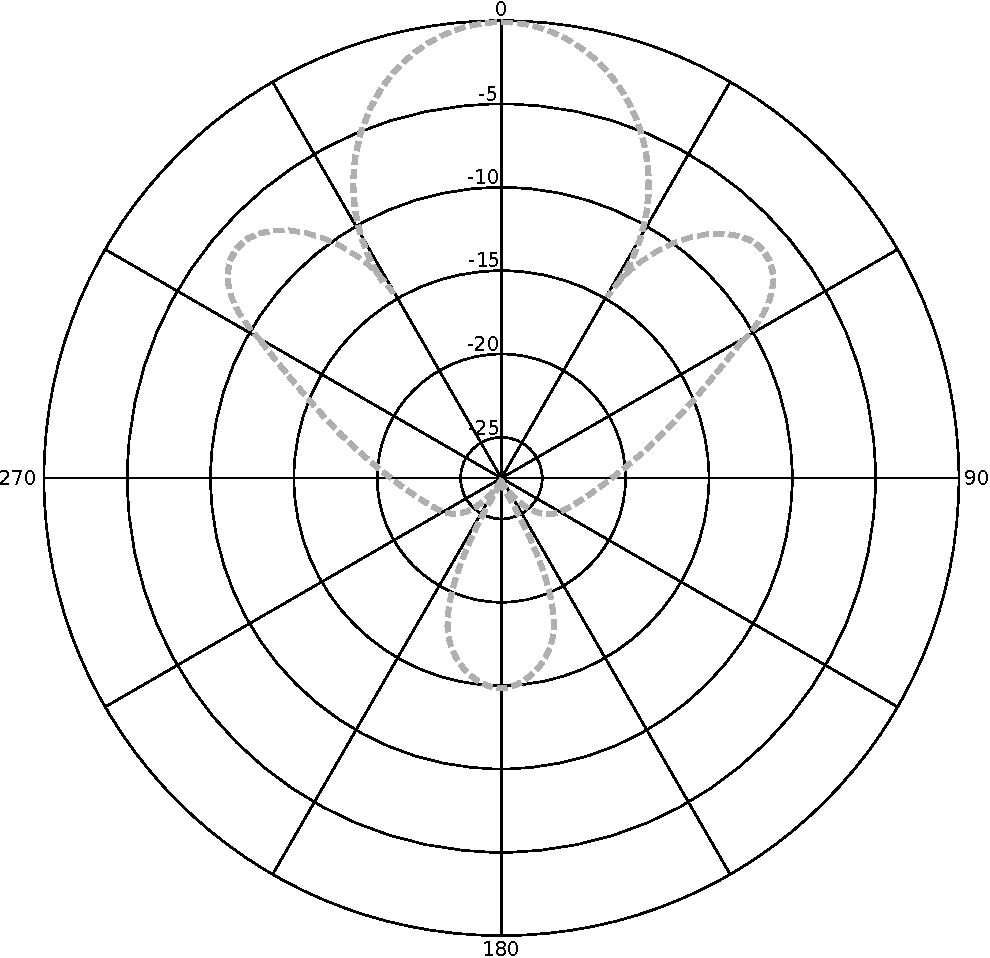
\includegraphics[width=0.4\textwidth]{02-background_and_motivation/img/antenna_pattern}

\caption{An example of an antenna-azimuth pattern, showing the gain in each
direction.\label{fig:02-Antenna_azimuth}}
\end{figure}


\begin{figure}
\centering

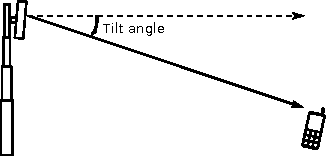
\includegraphics[width=0.6\textwidth]{02-background_and_motivation/img/antenna_tilt}

\caption{The antenna tilt, showing its angle with the horizontal plane. Adapted
from~\cite{WCDMAforUMTS_RadioAccessForThirdGenerationMobileCommunications}.\label{fig:02-Antenna-tilt}}
\end{figure}



\subsection*{Related work}

One of the approaches proposed by Gerdenitsch et al.~\cite{Antenna.tilt.and.CPICH:2003}
involves an ``ad-hoc'' strategy for adjusting antenna azimuth and
downtilt by analyzing the structure of the network. The objective
of this optimization was to improve the number of served users in
the target area. 

Siomina and Yuan~\cite{Antenna.Configuration:2008} proposed an approach
for automated optimization of antenna azimuth and tilt, including
support for both mechanical and electrical tilt. The implementation
introduced a SA-based algorithm that searches the solution space of
feasible antenna configurations. The goal of the optimization was
to improve power sharing among different cell channels and ultimately
improve the throughput of the network.

In~\cite{Antenna.azimuth.tilt:2009}, the authors presented a compound
optimization method containing two loops: the inner one and the outer
one. The inner loop concentrated on frequency planning while the outer
loop focused on finding the optimal settings of antenna azimuth and
tilt for the current solution delivered by the inner loop. This approach
is interesting because of its flexibility, e.g., the inner loop could
be replaced with some other optimization objective, like service coverage.

In~\cite{Eckhardt-Vertical_antenna_tilt_optimization_for_LTE:2011},
the authors proposed an autonomous optimization approach for the antenna
tilts. Based on the gradient-ascent method, the presented heuristic
showed the fast convergence needed for an online-optimization method
to be effective. 

\bigskip{}


Combining the power setting of the pilot signal with the antenna configuration
is also a common practice. For example, Siomina et al.~\cite{Coverage.optimization.on.CPICH.tilt.and.azimuth:2006}
present an optimization approach for maximizing the service coverage
that combines both antenna parameters with the power of the pilot
signal. Their SA-based algorithm searches the solution space of possible
configurations in order to improve the performance of the target radio
network by reducing the total interference. The simulation results
show the algorithm is capable of tackling large network instances.

Two optimization algorithms for finding an optimal setting of antenna
tilt and pilot-signal power were also introduced in the previously
cited work by Gerdenitsch et al.~\cite{Antenna.tilt.and.CPICH:2003}.
The first algorithm is based on a rule-based approach, while the second
one extends it by incorporating SA. The evaluation of both techniques
showed that the second algorithm achieves better solutions.

In a different work, Gerdenitsch et al.~\cite{GA.for.tilt.and.CPICH:2004}
proposed a genetic algorithm to tackle the optimization of antenna
tilt and pilot-signal power, the goal of which is to increase network
capacity. The implementation involves a deterministic fitness selection
scheme, a problem-specific recombination operator and an improved
mutation operator. After the initial identification of the best promising
individuals, a local-optimization technique is applied to improve
their fitness.


\section{Optimizing coverage \label{sec:Optimizing-coverage}}

Coverage is arguably the most common optimization objective considered
in radio-network optimization. A general objective function for coverage
optimization can be defined as follows:

\[
f_{\mathrm{cov}}=\frac{A_{\mathrm{covered}}}{A_{\mathrm{total}}},
\]


\noindent \nomenclature[S]{$A_{\mathrm{covered}}$}{Area under service coverage of the mobile network}\nomenclature[S]{$A_{\mathrm{total}}$}{Complete geographical area under optimization}

\noindent where $A_{\mathrm{covered}}$ represents the area covered
by the network and $A_{\mathrm{total}}$ represents the total area
under optimization. Thus, the expression $f_{\mathrm{cov}}$ represents
the proportion of the total area that is actually under network coverage,
the value of which ranges from 0 (no coverage) to 1 (total coverage).

The area under optimization is usually divided into squares (or pixels)
of a certain size, creating a Regular Square Grid (RSG\nomenclature[A]{RSG}{Regular square grid})
of a certain resolution. A pixel is considered covered if a given
QoS measure is above a defined threshold. It is also common to use
a binary function to check the coverage of a given pixel. The function
returns 1 if the pixel located at $(x,y)$ is covered, and 0 otherwise.


\subsection*{Related work}

Siomina and Yuan~\cite{Siomina:Minimum.pilot.power.for.service.coverage}
considered the problem of minimizing the pilot-signal power subject
to a coverage constraint. Their approach consists of an iterative
mathematical program, based on a linear-integer formulation of the
problem. The simulation results showed the trade-off between service
coverage and power consumption for different test networks.

Almaldi et al.~\cite{Amaldi-Radio_planning_and_coverage_optimization_of_3G_networks:2008}
investigated several mathematical-programming models for supporting
decisions on where to install new BSs and how to select their configuration
in order to find a trade-off between coverage and costs. The overall
model takes into account signal-quality constraints, in both uplink
and downlink directions, as well as the pilot-signal power.

Connecting UMTS and LTE-network optimization from the coverage point
of view, Sallent et al.~\cite{Sallent-A_roadmap_from_UMTS_to_LTE_optimization:2011}
presented a framework to automatically identify a cell with sub-optimal
coverage. The framework input is a collection of KPIs, including usage
statistics and UE field measurements. The authors used the experimental
results to provide a projection for the LTE self-optimization functionality.

In~\cite{Thampi-A_sparse_sampling_algorithm_for_self_optimization_of_coverage_in_LTE:2012},
the authors introduced a sparse-sampling algorithm to optimize the
coverage of LTE networks by means of antenna tilt. By applying a reinforcement-learning
technique, their approach optimizes coverage without prior knowledge
about the target network.

Parkinnen et al.~\cite{Coverage.optimization.with.cost.function:2002}
presented a gradient-descent method to minimize an objective function
that combines some KPIs with the service coverage. The power of the
pilot signal of the cells is periodically updated in order to improve
the aforementioned function.


\section{Discussion}

Regarding the optimization methods presented in the previous sections,
three distinctive groups emerge: genetic algorithms, linear programming
and other search methods.
\begin{description}
\item [{Genetic~algorithms}] These algorithms work on a population of
solutions, allowing a more comprehensive search for optimal solutions.
As a direct consequence, an increase in running time is commonly observed.
The implementation effort of genetic algorithms is to some degree
higher than for simpler search methods, e.g., local search, but their
inherent structure makes parallel implementations rather simple. Additionally,
genetic algorithms are less likely to be trapped in local optima,
since they are a population-based metaheuristic.
\item [{Linear~programming}] Linear-integer or mixed-integer programming
are widely used in different optimization areas and there are many
good software packages to solve such problems. Consequently, if a
problem can be modeled as a continuous linear problem, there is usually
no difficulty in finding optimality. In the context of this survey,
linear programming has proven useful for BS-location optimization
in early network planning stages.
\item [{Other~search~methods}] Other search methods, e.g., local search,
SA, tabu search or gradient descent, usually represent a compromise
between running time and quality of results. Their effectiveness relies
on evaluating a great number of alternative solutions. The number
of parameters taken into account, as well as the evaluation precision,
directly influence their running time. These methods do not excel
in full simulation scenarios. Moreover, some of them are easily trapped
in local minima.
\end{description}

\section{Summary}

The variety of optimization problems described in the previous sections
differ in many aspects, like implementation, running time and solution
quality. Picking the right method for a given situation depends on
the optimization task and the desired results. Since computational
time is usually an important restriction, simpler and faster methods
may be preferable.

Beside the convenience of a literature overview as presented here,
it is very important to develop a feeling for the properties, advantages
and drawbacks of the respective methods. Moreover, the recommendations
of experts regarding the interpretation of the solutions and the feedback
from everyday network operation are an essential input for establishing
high-quality optimization methods.

Additionally, as noted for some of the cited works, hybrid methods,
i.e., approaches that combine different optimization and/or search
techniques, usually give competitive solutions to complex optimization
problems. Therefore, a simple optimization algorithm can quickly find
a subset of reasonable solutions, whereas a more complex method could
be applied afterwards, to refine the search. Sometimes it may also
be useful to apply a local search method at the end to find better
solutions in the proximity of a current one.


\chapter{Principles of GPU Programming \label{chap:02-Principles_of_GPU_programming}}

During the past few years, the computing industry has been delivering
extra processing power in the form of parallel computing, i.e., more
cores instead of higher-frequency rates. Concurrently to this situation,
new hardware architectures have appeared. Among them is the programmable
Graphics Processing Unit (GPU\nomenclature[A]{GPU}{Graphics processing unit}),
the computing capacity of which is already showing a faster progress
compared to CPUs. The peak performance of the latest GPU is several
times higher than the latest CPU, but even more important is the trend~\cite{Cruz-How_to_obtain_efficient_GPU_kernels:2011}.

The GPU market was almost exclusively driven by the games industry.
This fact makes this commodity hardware cheaper than other alternatives
for High-Performance Computing (HPC\nomenclature[A]{HPC}{High-performance computing}),
e.g., the classic \textquoteleft{}mainframe\textquoteright{} servers.
Moreover, the performance-per-watt of GPUs is an extra benefit over
their raw performance~\cite{Cruz-How_to_obtain_efficient_GPU_kernels:2011}.

In February 2007, the first real opportunity for using GPUs for general
programming and scientific computing came about with the release of
the Compute Unified Device Architecture~(CUDA\nomenclature[A]{CUDA}{Compute unified device architecture})~\cite{CUDA}.

In the following, the focus on the CUDA architecture. In particular,
similar hardware produced by other vendors, e.g., AMD and Intel, as
well as other programming frameworks like OpenCL~\cite{Stone_OpenCL.A.parallel.programming.standard:2010},
are based on the same technology paradigm of massively-parallel processors.
For this reason, the principles presented in this section can be applied
to current GPU technologies, in a vendor-independent manner.


\section{CUDA \label{sec:02-CUDA}}

A GPU is effectively a large set of processor cores with the ability
to directly address into a global memory. This makes it easier for
developers to implement data-parallel kernels. The CUDA programming
model \cite{CUDA} was created for developing applications for the
GPU platform. A system within this model consists of a host, i.e.,
a traditional CPU, and one or more compute devices that are massively
data-parallel co-processors, i.e., a GPU. The host code transfers
data to and from the global memory of the GPU using CUDA-function
calls. Each processor of a CUDA device supports the Single-Program
Multiple-Data~(SPMD\nomenclature[A]{SPMD}{Single-program multiple-data})
model~\cite{Atallah-Algorithms_and_theory_of_computation:2002},
in which all concurrent threads are based on the same code, although
they may not follow exactly the same path of execution.

A CUDA program consists of multiple parts that are executed on either
the CPU or the GPU. For this reason, the CUDA programming model may
be viewed as an environment to isolate program parts that are rich
in data parallelism and thus should be executed on the GPU. The parallel
parts of a CUDA program are implemented as kernels, i.e., functions
written in the C language that describe the work of a single thread
of execution. Several restrictions apply on kernel functions: there
must be no recursion, no static variable declarations, and a non-variable
number of arguments~\cite{Ryoo-Optimization_principles_of_a_GPU_using_CUDA:2008}.
At run time, the kernel invocation is typically done on thousands
of threads, which are organized within developer-defined groups called
thread blocks. The threads can share data and synchronize their execution
only within the block they belong to. Thread blocks are, in turn,
organized in a higher-hierarchy level called grid. All threads within
a given grid execute the same kernel function. During execution, continuous
sections of threads within a block are grouped into warps of several
parallel threads (typically 32 or 64, depending on the target architecture),
which represent the multi-threading scheduling unit~\cite{Ryoo-Optimization_principles_of_a_GPU_using_CUDA:2008}.
A GPU contains several Streaming Multiprocessors (SMs\nomenclature[A]{SM}{Streaming multiprocessor}),
each of which executes one instruction at a time for all the 32 threads
in the warp. Consequently, if a thread block is not evenly divisible
by the warp size, any remaining thread slots are wasted. Another undesirable
situation appears when threads in a warp take different control paths,
since the execution performance of the entire warp is reduced.

\begin{figure}
\centering

\includegraphics[width=0.4\textwidth]{02-background_and_motivation/img/GPU_architecture}

\caption{A simplified diagram of the architecture of a modern GPU. Adapted
from~\cite{Ryoo-Optimization_principles_of_a_GPU_using_CUDA:2008}.\label{fig:02-GPU_architecture}}
\end{figure}


The architecture of a typical GPU is depicted in Figure~\ref{fig:02-GPU_architecture}.
It consists of $n$ SMs, each containing $m$ Streaming Processors
(SPs\nomenclature[A]{SP}{Streaming processor}). Each SP executes
a single instruction of a thread in a Single-Instruction, Multiple-Thread
(SIMT\nomenclature[A]{SIMT}{Single instruction multiple thread})
manner~\cite{Cruz-How_to_obtain_efficient_GPU_kernels:2011}. The
registers of each SM are dynamically partitioned among the threads
running on it. 

Table~\ref{tab:02-GPU_memory_properties} lists the different types
of memory on a GPU, along with some of their properties. Specifically,
the location of the memory, its hit-latency in terms of clock cycles,
whether it is read-only or not, and the program scope it may be accessed
from. Due to the different memory system a GPU has, the actual throughput
an application can achieve depends on issues related to the access
to memory, in particular the slow accesses to global memory from the
GPU chip, and the use of shared memory in the SPs to mitigate the
high-latency effects~\cite{Cruz-How_to_obtain_efficient_GPU_kernels:2011}.
Since variables in the source code can be declared to reside in global,
shared, local, or constant memory, a programmer has the means to organize
the code in such a way that the application throughput can be maximized.

\begin{table}
\caption{Properties of different memory types on a GeForce 8800 GPU. Adapted
from~\cite{Ryoo-Optimization_principles_of_a_GPU_using_CUDA:2008}.\label{tab:02-GPU_memory_properties}}


\centering

\begin{tabular}{lllll}
\hline 
Memory & Location & Latency & Read-only & Program scope\tabularnewline[\doublerulesep]
\hline 
Global & off-chip & 200-300 cycles & no & global\tabularnewline
Texture & on-chip cache & >100 cycles & yes & global\tabularnewline
Shared & on-chip & >1 cycle & no & function\tabularnewline
Register & on-chip & \textasciitilde{}1 cycle & no & function\tabularnewline
\hline 
\end{tabular}
\end{table}


Clearly, there are hard limits to the memories, threads, and total
bandwidth available to an application running on a GPU. Managing these
limits is critical when optimizing applications, but applying strategies
for avoiding one limit can easily cause other limits to be hit. Additionally,
managing the behavior of threads so that those in the same warp follow
the same control paths and load contiguous values from global memory
can improve the execution performance~\cite{Ryoo-Optimization_principles_of_a_GPU_using_CUDA:2008}.

A detailed discussion of the CUDA programming model can be found in~\cite{Farber-CUDA_application_design_and_development:2011}.


\section{OpenCL \label{sub:02-OpenCL}}

The Open computing language (OpenCL)~\cite{Stone_OpenCL.A.parallel.programming.standard:2010}
is an open parallel computing API designed to enable GPUs and other
co-processors to work together with the CPU, providing additional
computing power. As a standard, OpenCL 1.0 was released in 2008, by
The Khronos Group, an independent standards consortium~\cite{Munshi_The.OpenCL.specification:2009}.

The main advantage of OpenCL over CUDA relies on the fact that its
source code can be compiled to run on a variety of hardware, including
multicore CPUs and GPUs from different vendors. This provides a complete
framework that is capable of exploiting the parallel features of different
hardware without the need of changing the implementation. Moreover,
being an open standard, its users are not tight to the decision of
only one vendor. As it was mentioned before, the details described
in the previous sections may be equally applied on CUDA and OpenCL.

One unfortunate consequence of the vendor variety is that CUDA and
OpenCL have each introduced its own naming conventions. For the sake
of consistency, in Table~\ref{tab:02-CUDA_OpenCL_translation}, a
short ``translation dictionary'' between both platforms is presented.

\begin{table}
\caption{Naming-convention translation between OpenCL and CUDA. Adapted from~\cite{Kloeckner_CUDA.OpenCL.dictionary:2011}.\label{tab:02-CUDA_OpenCL_translation}}


\centering

\begin{tabular}{r|l}
\hline 
\textbf{OpenCL} & \textbf{CUDA}\tabularnewline[\doublerulesep]
\hline 
Grid & Grid\tabularnewline
Work group & Block\tabularnewline
Work item & Thread\tabularnewline
\_\_kernel & \_\_global\_\_\tabularnewline
\_\_global & \_\_device\_\_\tabularnewline
\_\_local & \_\_shared\_\_\tabularnewline
\_\_private & \_\_local\_\_\tabularnewline
image\emph{n}d\_t & texture<type,\emph{n},...>\tabularnewline
barrier(L|M|F) & \_\_syncthreads( )\tabularnewline
get\_local\_id(0|1|2) & threadIdx.x|y|z\tabularnewline
get\_group\_id(0|1|2) & blockIdx.x|y|z\tabularnewline
get\_global\_id(0|1|2) & \emph{(not implemented)}\tabularnewline
\hline 
\end{tabular}
\end{table}


In the remainder of this thesis, the naming convention introduced
by the CUDA platform is used.


\section{Summary}

This chapter gave an overview of the basic concepts, the potential
and the limitations of the GPUs when used as parallel processors for
general programming. In particular, emphasis has been given to the
details that differentiate this platform from CPUs. In this sense,
it is important to recognize which applications can benefit from using
a GPU and which not, also taking into consideration the effort required
at the implementation time.
